\section{Extra\c{c}\~ao de par\^ametros com \texttt{fsolve}}\label{sec:extracao}

O datasheet n\~ao d\'a $R_s$, $R_p$, $I_0$ nem $E_g$. D\'a s\'o pontos de opera\c{c}\~ao. Este
cap\'itulo mostra como transformar esses pontos nos par\^ametros do modelo. Arquivos:
\arq{painel/extrair_parametros.m},
\arq{painel/identificabilidade_2d.m}, \arq{painel/validar_painel.m}.

\begin{figure}[htbp]
\centering
\begin{tikzpicture}
  \node[bloco,minimum width=2.7cm] (ds) at (0,0) {\textbf{Datasheet}\\{\scriptsize $I_{sc},V_{oc},I_{mp},V_{mp}$}\\{\scriptsize $K_v$}};
  \node[bloco,minimum width=2.7cm] (re) at (3.9,0) {\textbf{5 res\'iduos}\\{\scriptsize \texttt{kcl\_modulo} em}\\{\scriptsize $I_{sc}$, $V_{oc}$, MPP,}\\{\scriptsize $dP/dV$, $K_v$}};
  \node[ctrl,minimum width=2.7cm] (lm) at (7.8,0) {\textbf{\texttt{fsolve}}\\{\scriptsize Newton com regi\~ao de}\\{\scriptsize confian\c{c}a (dogleg)}};
  \node[bloco,minimum width=2.7cm] (pa) at (11.7,0) {\textbf{Par\^ametros}\\{\scriptsize $I_{pv},I_{01},R_s,R_p$}\\{\scriptsize e $E_g$ efetivo}};
  \node[dest,minimum width=2.7cm] (va) at (11.7,-3) {\textbf{Valida\c{c}\~ao}\\{\scriptsize $\gamma_P$ fora do ajuste}\\{\scriptsize KC200GT $\times$ Villalva}};
  \draw[seta] (ds) -- (re);
  \draw[seta] (re) -- (lm);
  \draw[seta] (lm) -- (pa);
  \draw[seta] (lm.south) -- ++(0,-0.9) -| node[rot,above,pos=0.25]{repete at\'e $\|r\|<10^{-6}$} (re.south);
  \draw[seta] (pa) -- (va);
\end{tikzpicture}
\caption{Pipeline da extra\c{c}\~ao. O \texttt{fsolve} chama os res\'iduos quantas vezes forem
necess\'arias; a valida\c{c}\~ao usa o coeficiente de $P_{max}$, que n\~ao entra no ajuste.}
\label{fig:extracao}
\end{figure}

\subsection{5 inc\'ognitas, 5 condi\c{c}\~oes}

As inc\'ognitas s\~ao $x=[\Ipv,\ \log_{10}I_{01},\ R_s,\ R_p,\ E_g]$ (com $R_s$ e $R_p$ do
m\'odulo inteiro). As cinco condi\c{c}\~oes v\^em do datasheet; cada uma vira um res\'iduo
calculado com \arq{kcl_modulo}:

\begin{align}
F_1&=F(0,\Isc)=0 &&\text{(curto-circuito)}\\
F_2&=F(\Voc,0)=0 &&\text{(circuito aberto)}\\
F_3&=F(\Vmp,\Imp)=0 &&\text{(o MPP est\'a na curva)}\\
F_4&=\Imp+\Vmp\,\dfrac{dI}{dV}\Big|_{mp}=0 &&\text{(o MPP \'e m\'aximo: } dP/dV=0)\\
F_5&=F\big(\Voc+K_v\Delta T,\,0\big)\ \text{em } T_n+\Delta T=0,\ \Delta T=25\,\text{K} &&\text{(coeficiente de }V_{oc}\text{)}
\end{align}

Todos os res\'iduos s\~ao divididos por $\Isc$, para ficarem na mesma escala. Como h\'a 5
equa\c{c}\~oes e 5 inc\'ognitas, o ajuste \'e na verdade a solu\c{c}\~ao de um sistema; se tudo
der certo, o res\'iduo final \'e praticamente zero. O c\'odigo exige menos de $10^{-6}$ e emite
\texttt{warning} se n\~ao convergir. $E_g$ \'e inc\'ognita porque a condi\c{c}\~ao 5 \'e a \'unica
que enxerga a temperatura, e $E_g$ controla como $I_0$ varia com $T$.

\codigo{painel/extrair_parametros.m}{87}{109}{os cinco res\'iduos, um por condi\c{c}\~ao do datasheet.}{lst:residuos}

\begin{logica}
\begin{enumerate}
\item \texttt{aplicar\_incognitas(x,p0)} converte o vetor $x$ num \emph{struct} de par\^ametros
 por c\'elula: $I_{01}=10^{x_2}$, $I_{02}=\text{raz\~ao}\cdot I_{01}$, $R_s=x_3/N_s$, $R_p=x_4/N_s$.
\item As linhas 1 a 3 apenas perguntam: ``o ponto $(V,I)$ do datasheet satisfaz a equa\c{c}\~ao do
 m\'odulo?'' A resposta \'e o res\'iduo de \arq{kcl_modulo}.
\item \texttt{F4} usa a inclina\c{c}\~ao devolvida por \arq{kcl_modulo} (terceira sa\'ida) para
 impor $dP/dV=0$ no MPP.
\item \texttt{F5} refaz a pergunta a 50\,$^\circ$C, com $V_{oc}$ deslocado de $K_v\cdot25$. Como
 $T$ muda, quem responde \'e a lei de $I_0(T)$, ou seja, o $E_g$.
\item O vetor final \'e normalizado por $\Isc$.
\end{enumerate}
\end{logica}

\subsubsection{Por que o segundo diodo \'e fixado (D9)}

Se $I_{02}$ \'e fixado em qualquer valor entre $10^{-12}$ e $10^{-5}$\,A, as quatro condi\c{c}\~oes
de STC continuam fechando exatamente: falta informa\c{c}\~ao. Adota-se ent\~ao a hip\'otese
publicada de Ishaque et al.\ (2011): $a_1=1$, $a_2=1{,}2$ e $\boldsymbol{I_{01}=I_{02}}$. O modelo
de 1 diodo (\texttt{'1d'}, com $a=1{,}1$ e $I_{02}=0$) tamb\'em existe, para compara\c{c}\~ao.

\subsubsection{Vari\'aveis do solver e chute inicial}

O \texttt{fsolve} n\~ao aceita limites. As vari\'aveis do solver s\~ao $y=[\Ipv,\ \log_{10}I_{01},\ \log_{10}R_s,\ \log_{10}R_p,\ E_g]$,
e o c\'odigo converte de volta com $R_s=10^{y_3}$ e $R_p=10^{y_4}$ antes de calcular os res\'iduos.

\begin{center}\small
\begin{tabular}{@{}lcp{7.6cm}@{}}
\toprule
Vari\'avel & Chute inicial & Motivo \\ \midrule
$\Ipv$ & $\Isc$ & No curto $\Isc=\Ipv-$perdas, ent\~ao $\Ipv$ fica um pouco acima de $\Isc$ \\
$\log_{10}I_{01}$ & $-8$ & $I_{01}$ varia muitas d\'ecadas; em log as vari\'aveis ficam na mesma ordem \\
$\log_{10}R_s$ & $\log_{10}0{,}2$ & $R_s=10^{y}$ \'e sempre positivo \\
$\log_{10}R_p$ & $\log_{10}300$ & Idem \\
$E_g$ [eV] & 1,12 & Gap do sil\'icio como ponto de partida \\
\bottomrule
\end{tabular}
\end{center}

\begin{atencao}[: por que o log em $R_s$ e $R_p$]
Testado: com as vari\'aveis diretas e o mesmo chute, o \texttt{fsolve} \textbf{divergiu no ZTP-160M} (1 e 2 diodos): $R_p$ foi para $-4{,}5\times10^{12}\,\Omega$ e o
res\'iduo parou em $4\times10^{-2}$ ap\'os 500 itera\c{c}\~oes. No KC200GT funcionava. Em $\log_{10}$, a diverg\^encia para valores negativos some, e o \texttt{fsolve}
convergiu nos quatro casos (ZTP-160M e KC200GT, 1 e 2 diodos) para os mesmos par\^ametros do m\'etodo anterior (LM pr\'oprio com limites), com res\'iduo de $\sim10^{-15}$.
\end{atencao}

\subsection{Como o \texttt{fsolve} resolve o sistema}

Um sistema de 5 equa\c{c}\~oes e 5 inc\'ognitas, $r(y)=0$, \'e resolvido por \textbf{Newton}: em cada itera\c{c}\~ao aproxima-se $r$ por uma reta (em v\'arias vari\'aveis, pela
matriz jacobiana $J$) e salta-se para onde ela cruza o zero:
\begin{equation}\label{eq:newton}
J\,\Delta y=-r,\qquad y\leftarrow y+\Delta y .
\end{equation}
Newton puro converge muito r\'apido perto da solu\c{c}\~ao, mas longe dela um passo pode lan\c{c}ar uma vari\'avel para um valor absurdo (aqui, com exponenciais, isso estoura).
O algoritmo padr\~ao do \texttt{fsolve} \'e uma \emph{regi\~ao de confian\c{c}a} (\emph{dogleg}): ele limita o tamanho do passo a uma regi\~ao onde confia na aproxima\c{c}\~ao linear, e s\'o
aceita o passo se o res\'iduo realmente diminuir; sen\~ao encolhe a regi\~ao e tenta de novo. O jacobiano \'e estimado por diferen\c{c}as finitas, ent\~ao n\~ao precisamos
derivar \texttt{kcl\_modulo} em rela\c{c}\~ao a cada par\^ametro.

\codigo{painel/extrair_parametros.m}{46}{64}{vari\'aveis em log, chamada do \texttt{fsolve} e montagem do resultado.}{lst:fsolve}

\begin{logica}
\begin{enumerate}
\item \texttt{y0}: chute inicial das vari\'aveis do solver (tabela acima).
\item \texttt{fun = @(y) residuos\_extracao([...])}: um \emph{handle} que converte $y$ em $x=[\Ipv,\log I_{01},R_s,R_p,E_g]$ (com $R_s=10^{y_3}$, $R_p=10^{y_4}$) e devolve os 5 res\'iduos.
\item \texttt{optimoptions('fsolve',...)}: toler\^ancias de $10^{-14}$ e at\'e 500 itera\c{c}\~oes e 5000 avalia\c{c}\~oes, porque o sistema tem solu\c{c}\~ao exata (res\'iduo $\approx0$) e queremos
 ela, n\~ao s\'o uma aproxima\c{c}\~ao.
\item \texttt{fsolve(fun, y0, opcoes)} devolve a solu\c{c}\~ao \texttt{y}, o vetor de res\'iduos \texttt{r} e informa\c{c}\~oes do solver (\texttt{saida.iterations}).
\item O resultado volta para $x$ e vira o \emph{struct} de par\^ametros por c\'elula com \texttt{aplicar\_incognitas}. \texttt{info.residuo = norm(r)} \'e conferido depois: abaixo de $10^{-6}$ \'e
 aceito, sen\~ao h\'a \texttt{warning}.
\end{enumerate}
\end{logica}

\begin{resumo}
O \texttt{fsolve} \'e da Optimization Toolbox. O projeto passa a depender dela, e n\~ao roda mais s\'o com MATLAB base. Antes, um Levenberg--Marquardt pr\'oprio (com limites e
50 linhas) fazia o mesmo papel; foi removido junto com o seu teste.
\end{resumo}

\subsection{Valida\c{c}\~ao em duas etapas}

\textbf{Primeiro no KC200GT.} Antes de confiar no m\'etodo, ele foi aplicado a um painel cujo
resultado \'e publicado (Kyocera KC200GT, Villalva 2009); o teste est\'a em
\arq{tests/test_extracao.m}.

\textbf{Depois no ZTP-160M, sem curvas.} Como o datasheet n\~ao tem curvas I-V, os pontos de STC
s\'o confirmam que o ajuste fechou. A valida\c{c}\~ao \emph{independente} \'e o coeficiente
t\'ermico de $P_{max}$, que n\~ao entra no ajuste:

\begin{resultado}
\small\centering
\begin{tabular}{@{}lcccc@{}}
\toprule
Modelo & Erro $P_{max}$ (STC) & Erro $V_{oc}$ & $\gamma_P$ do modelo & $\gamma_P$ datasheet \\ \midrule
1 diodo & $+0{,}296$\,\% & $-0{,}032$\,\% & $-0{,}366$\,\%/K & $-0{,}4$\,\%/K \\
2 diodos & $+0{,}296$\,\% & $-0{,}032$\,\% & $-0{,}363$\,\%/K & $-0{,}4$\,\%/K \\
\bottomrule
\end{tabular}
\end{resultado}

O erro de 0,3\,\% em $P_{max}$ n\~ao \'e do modelo: o datasheet \'e inconsistente
($V_{mp}I_{mp}=160{,}47$\,W, mas $P_{max}=160$\,W). O ajuste imp\~oe $(V_{mp},I_{mp})$, e contra
$V_{mp}I_{mp}$ o erro \'e de $8\times10^{-5}$\,\%. O $\gamma_P$ previsto \'e cerca de 9\,\% menor em
m\'odulo que o do datasheet; o relat\'orio declara essa diferen\c{c}a como limita\c{c}\~ao.

\subsection{Identificabilidade do segundo diodo (E1)}

Para mostrar que o datasheet n\~ao fixa $I_{02}$, refaz-se a extra\c{c}\~ao com $I_{02}/I_{01}\in\{0{,}01;\,0{,}1;\,1;\,10;\,100\}$.
Todas fecham, e o que muda \'e a previs\~ao fora de STC:

\begin{center}\small
\begin{tabular}{@{}rcccc@{}}
\toprule
$I_{02}/I_{01}$ & Res\'iduo & $E_g$ efetivo [eV] & $\eta(200)/\eta(\text{STC})$ & $\gamma_P$ [\%/K] \\ \midrule
0,01 & $2\times10^{-11}$ & 1,307 & 94,83\,\% & $-0{,}3623$ \\
0,1 & $3\times10^{-11}$ & 1,307 & 94,82\,\% & $-0{,}3624$ \\
1 & $5\times10^{-11}$ & 1,304 & 94,79\,\% & $-0{,}3628$ \\
10 & $5\times10^{-8}$ & 1,274 & 94,45\,\% & $-0{,}3664$ \\
100 & $3\times10^{-8}$ & 1,164 & 93,08\,\% & $-0{,}3743$ \\
\bottomrule
\end{tabular}
\end{center}

Todos os res\'iduos s\~ao muito menores que $10^{-6}$: todos os modelos satisfazem o datasheet. Mas
a efici\^encia em baixa luz vai de 94,8\,\% a 93,1\,\%. Essa faixa de menos de 2 pontos percentuais
\'e a \textbf{incerteza que o datasheet deixa} em baixa irradi\^ancia, pequena frente aos efeitos
estudados depois (9\,\%, 11\,\% e 22\,\% na energia). Por isso a escolha da raz\~ao 1 n\~ao
contamina as conclus\~oes.

\begin{figure}[htbp]
\centering
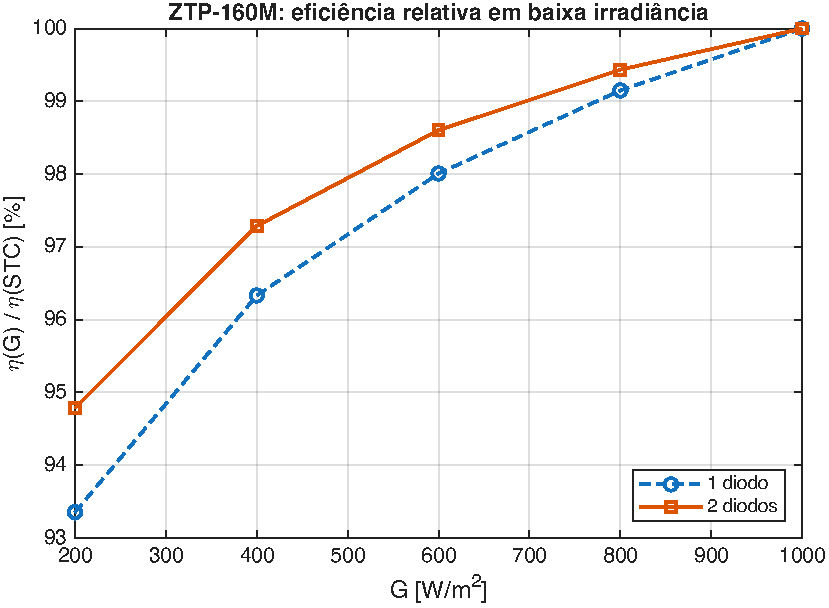
\includegraphics[width=0.48\linewidth]{e1_eficiencia_relativa.pdf}\hfill
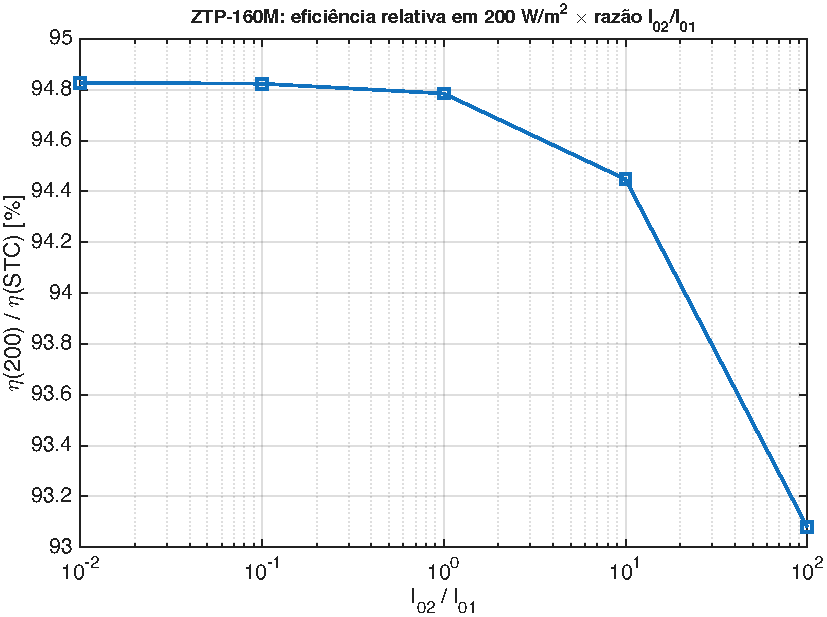
\includegraphics[width=0.48\linewidth]{e1_identificabilidade.pdf}
\caption{E1. Esquerda: efici\^encia relativa $\eta(G)/\eta(\text{STC})$ nos modelos de 1 e 2
diodos. Direita: efici\^encia em 200\,W/m$^2$ em fun\c{c}\~ao de $I_{02}/I_{01}$.}
\label{fig:e1}
\end{figure}
